%!TEX root = ../main.tex

\section{Results}
\label{s:results}

\subsection{Fake versus real normals}
	\todo[inline]{Show results of PN triangles with fake and real normals, and discuss differences}
	\todo[inline]{Computational complexity of the fake normals and the real normals, consider one triangle.}
	\todo[inline]{Any unsolved problems?}

\iftoggle{PHONG}{
\subsection{Phong tesselation versus PN triangles}
	\future{Show comparison of Phong tesselation with PN triangles: performance, visual results, continuity, probably in cooperation with Jelle and Gerben}
	\future{Any unsolved problems?}
}

\begin{figure*}
	\plaatje{Roteer onze rendering zodat hij klopt met de blauwe rendering}
	\centering
	\begin{subfigure}[b]{0.2\textwidth}
		\centering
		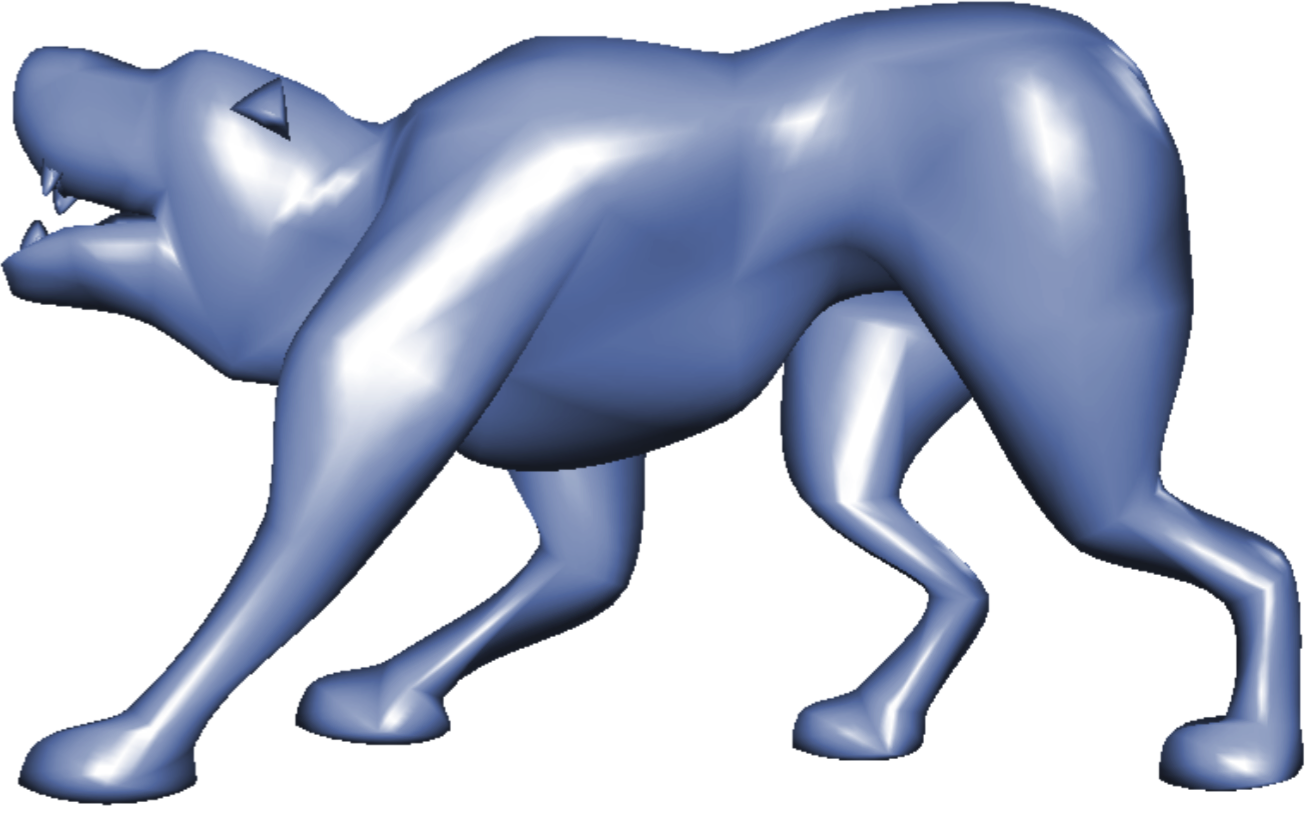
\includegraphics[width=\textwidth]{content/img/results/dogCPU.png}
		\caption{Dog on CPU}
		\label{fig:results:cpugpu:cpuDog}
	\end{subfigure}
	\hspace{0.1\textwidth}
	\begin{subfigure}[b]{0.2\textwidth}
		\centering
		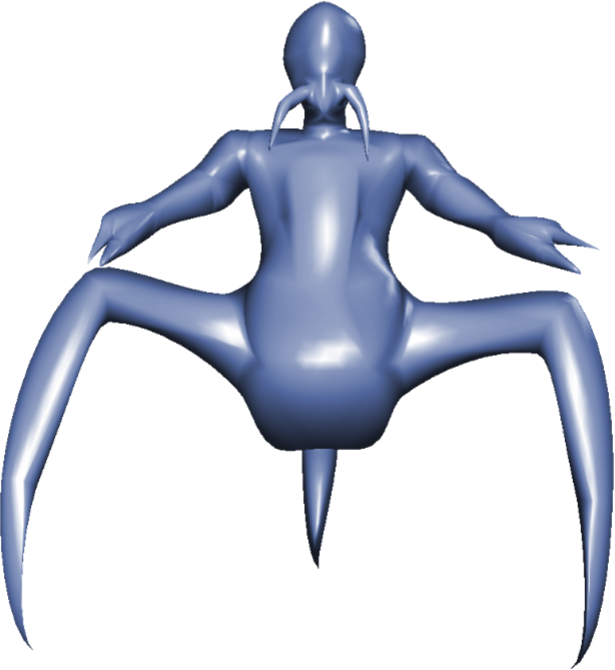
\includegraphics[width=\textwidth]{content/img/results/voreCPU.png}
		\caption{Vore on CPU}
		\label{fig:results:cpugpu:cpuVore}
	\end{subfigure}	
	\hspace{0.1\textwidth}
	\begin{subfigure}[b]{0.2\textwidth}
		\centering
		\includegraphics[width=\textwidth]{content/img/results/shamblercpu.png}
		\caption{Vore on cpu}
		\label{fig:results:cpugpu:cpuShambler}
	\end{subfigure}		

	\begin{subfigure}[b]{0.2\textwidth}
		\centering
		\includegraphics[width=\textwidth]{content/img/results/doggpu.png}
		\caption{Dog on GPU}
		\label{fig:results:cpugpu:gpuDog}
	\end{subfigure}
	\hspace{0.1\textwidth}
	\begin{subfigure}[b]{0.2\textwidth}
		\centering
		\includegraphics[width=\textwidth]{content/img/results/voregpu.png}
		\caption{Vore on GPU}
		\label{fig:results:cpugpu:gpuVore}
	\end{subfigure}	
	\hspace{0.1\textwidth}
	\begin{subfigure}[b]{0.2\textwidth}
		\centering
		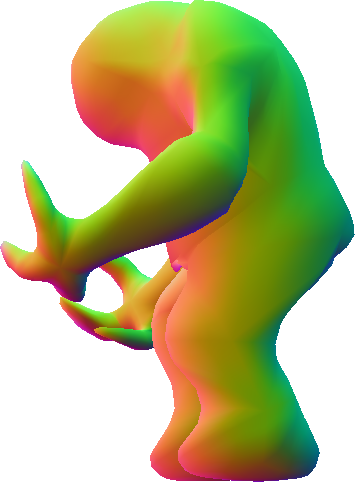
\includegraphics[width=\textwidth]{content/img/results/shamblerGPU.png}
		\caption{Vore on GPU}
		\label{fig:results:cpugpu:gpuShambler}
	\end{subfigure}			
	\caption{A family of game characters from the game Quake 1. \subref{fig:results:cpugpu:cpuDog}, \subref{fig:results:cpugpu:cpuVore} and \subref{fig:results:cpugpu:cpuShambler} are rendered on a CPU by \citeauthor{vlachos2001curved}. \subref{fig:results:cpugpu:gpuDog}, \subref{fig:results:cpugpu:gpuVore}, \subref{fig:results:cpugpu:gpuShambler} are rendered by our implementation. Figures \subref{fig:results:cpugpu:cpuDog}, \subref{fig:results:cpugpu:cpuVore} and \subref{fig:results:cpugpu:cpuShambler} were taken from \textcite{vlachos2001curved}.}
	\label{fig:results:cpugpu}
\end{figure*}

\subsection{Pipeline}
	\Cref{fig:results:cpugpu} shows the rendering by \citeauthor{vlachos2001curved} next to our rendering of, probably, the same model. The only difference between these two models should be the pattern in which the triangles of the input mesh are subdivided into flat triangles. A visual inspection shows no obvious differences between the models, leading us to suggest that the difference in triangulation does not matter much. 